\chapter{Methodology}
\label{ch_methodology}

%This is what I did to test and confirm my hypothesis.


%You may want to split this chapter into sub chapters depending on your design. I suggest you change
%the title to something more specific to your project.

%This is where you describe your design process in detail, from component/device selection to actual
%design implementation, to how you tested your system. Remember detail is important in technical
%writing. Do not just write I used a computer give the computer specifications or the oscilloscopes part
%number. Describe the system in enough detail so that someone else can replicate your design as well
%as your testing methodology.

%If you use or design code for your system, represent it as flow diagrams in text.

\section{Outline}

This study aims to investigate the performance of readily available parts for the purposes of creating a laser tag system. The following chapter presents the methodology that was followed to test the performance of the various modules and the system as a whole in the context of the intended use case (laser tag). A phased approach was taken in the method of investigation.

\begin{figure}[H]
	\centering
	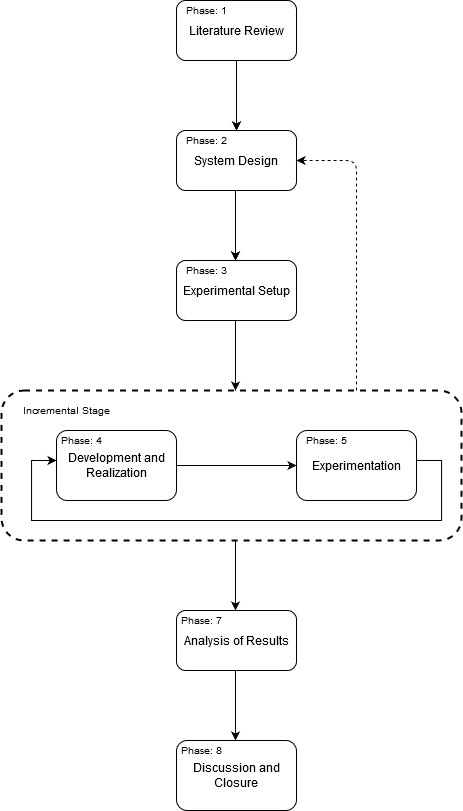
\includegraphics[width=0.5\textwidth]{figures/methodology/methodology}
	\caption{Methodology Flow Diagram}
	\label{fig:methodology_overview}
\end{figure}


The first phase involves investigating the relevant literature. The system design follows the literature review and chapter \ref{ch_design} has been dedicated to this phase of the investigation. The third phase is the experimental setup which covers the test and measurement equipment used during the investigation and covers component selection and reasoning. Following the third phase is an iterative stage which begins with phase 4 development and realization and leads into the experimentation phase. The experimentation phase feeds back to the development stage allowing for incremental improvement to the system design.

The second last phase is the analysis of results, chapter \ref{ch_results} has been dedicated to this. The final phase comprises the discussion and closure, which has been split across chapters \ref{ch_discussion} through \ref{ch_recommendations}.

%Finally the testing methodology is covered. Testing was performed in two phases, the first phase involves testing of individual modules. This modular testing is analogous to unit-tests in the computer programming paradigm. The second phase of testing involves characterising the performance of the final system prototype.

\section{Phase 1 - Literature}

Lit review

Questions:

\begin{itemize}
	\item What methods exist for detection of light?
	\item ?
\end{itemize}


%%%%%%%%%%%%%%%%%%%%

\section{Phase 2 - Design}

The project can be divided into two subsystems. The tagger (transmitter) and the target (receiver). These subsystems can be further subdivided into their respective software and hardware modules. Chapter \ref{ch_design} goes into detail on the design of these components.

\begin{figure}[H]
	\centering
	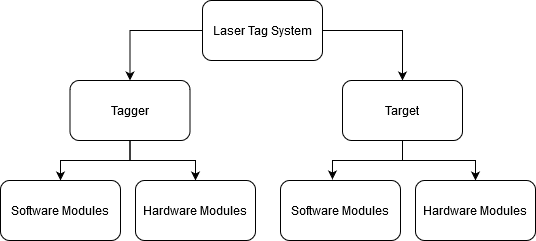
\includegraphics[width=0.7\linewidth]{figures/methodology/design_overview}
	\caption{Design Overview}
	\label{fig:designoverview}
\end{figure}

Figure \ref{fig:designoverview} provides a breakdown of the systems high-level design requirements.


%%%%%%%%%%%%%%%%%%%%

\section{Test and Measurement Equipment}

\subsection{Power Supply}
Access to the university laboratory equipment is limited.

A large potion of the testing will be done using a custom built power supply, created from an ATX PSU. The particular unit that was repurposed was a 280W LiteOn PSU. This unit is capable of supplying $\pm$ 12V, $\pm$ 5V, and 3.3V.

On occasion when a variable power supply was required, XXX

\subsection{Measurement}

Experiments requiring the use of an oscilloscope used a combination of the XXX Picoscope which I had access to while at home or the XXX which I used while in the university labs.

For debugging and general purpose measurements the fragram T2612 multimeter was used.



%%%%%%%%%%%%%%%%%%%%

\section{Hardware Components}

\subsection{UCT STM32F0 Development Board}
The STM32F051C6 microcontroller was chosen due to its combination of low cost and availability. UCT has a custom design development board centred on this microcontroller. The final prototype is centred purely on the STM32F0 microcontroller and bare-bones supporting circuity, however a vast amount of the testing was done on the development board hence its inclusion in this section.

\subsubsection{ADC Peripheral}

\subsubsection{ADC DMA}

\subsection{Arduino}
The Arduino platform was used whenever for various quick prototyping where unofficial testing was required. This is because the Arduino platform has many well established libraries and a simplified development environment which allowed for faster prototyping.

\subsection{Power IR LED}

The LZ1-10R702 high power, PCB mounted LED from LedEngin Inc. was used to produce the required 940nm wavelength infrared radiation. To ensure proper heat dissipation generic adhesive based heat-sink was attached to the module.

\subsection{Operational Amplifier}
xxx

\subsection{LED Current Regulator}
xxx
IRLZ44NPBF N-Channel MOSFET from Infineon



%%%%%%%%%%%%%%%%%%%%

\section{Software Applications}

\subsection{STM32 CubeIDE}
ST microelectronics provides a custom version of the Eclipse IDE, distributed under the name CubeIDE. This is an all in one integrated developer environment for STM32 microcontrollers. Version 1.3.0 was used for the software development in this study.

CubeIDE provides a 'Device Configuration Tool' along with an official library called HAL (Hardware Abstraction Layer). The combination of the configuration tool and HAL library helped speed up the software development. The CubeIDE also includes a debug tool with direct register/memory access which assisted with debugging.

XXX -talk about LCD libary

\subsection{Arduino IDE}
The Arduino IDE provides a very compact but elegant serial monitor which was used for serial communication between the STM32F0 microcontroller and the PC for the purposes of debugging.

In addition, any Arduino specific software development was done using the Arduino IDE.

\subsection{Git}



%%%%%%%%%%%%%%%%%%%%

\section{Testing Methodology}

\subsection{LED Driver}
The following tests were performed...


\subsection{Tests $\setminus$ Results to gather}
\textbf{Hardware}
\begin{itemize}
	\item IR Power LED:
	\begin{itemize}
		\item Beam angle (focus vs no focus)
		\item Beam strength (LUX)
		\item LED Current draw
		\item LED temperature (basic sensor or a temperature gun that I borrow from somewhere)
		\item MOSFET temperature
	\end{itemize}
	\item For each photo-sensor (photodiode, phototransistor, all in one receiver module):
	\begin{itemize}
		\item Receiving beam-angle
		\item Output signal strength vs light-intensity/distance
		\item Reaction time (rise time)
	\end{itemize}
	\item Op-Amp:
	\begin{itemize}
		\item Op-amp gain performance (push to limit) (at 36kHz)
		\item Op-amp frequency performance (at some fixed gain)
		\item Filter performance (anti-aliasing and high pass filtering)
	\end{itemize}
\end{itemize}

\textbf{Software}
\begin{itemize}
	
	\item Transmitter
	\begin{itemize}
		\item Timing accuracy
	\end{itemize}

	%\item Protocol
	%\begin{itemize}
	%	\item
	%\end{itemize}
	
	\item Receiver
	\begin{itemize}
		\item Bit error rate / max receiver distance - (not sure how I will implement this yet)
		\item Bit error correction - (not sure how I might implement this yet)
		\item Modulation to High/Low logic value [DSP processing analysis]
		\begin{itemize}
			\item Latency
			\item Testing the timing between stages of demodulating and decoding
		\end{itemize}
	\end{itemize}

\end{itemize}









